% this main.tex largely serves to boot up all the packages and tie the various files together 

% add 'twocolumn' as an option in [] to get two columns, if you want
\documentclass[12pt,oneside,a4paper]{report}


% PACKAGES --------------------
% if this becomes too much, full install of latex, put in filename.sty in same folder as main.tex
% include \ProvidesPackage{packagename} and use usepackage{that} here

\usepackage[english]{babel}
\usepackage[utf8]{inputenc}

%next 4 lines suppress "Chapter N" etc. which is obnoxious
\usepackage{titlesec}
\usepackage{lipsum}

\titleformat{\chapter}[display]
{\normalfont\bfseries}{}{0pt}{\Large} %or {\Huge}

\usepackage{graphicx}  % use this to handle images

%FIXME!! GRAPHICSPATH DOESNT WORK
%\graphicspath{ {/home/pat/heme-binding/thesis/figures/} } % specify path to images
%\graphicspath{figures/}
%\graphicspath{./figures/}
% none of these work. manually specifying figures/figuretitle works...


%\usepackage{xcolor}
% for the uh, apparently American style of quotation marks
\usepackage [english]{babel}
\usepackage [autostyle, english = american]{csquotes}

\MakeOuterQuote{"} % or `` and " or ` and '


\usepackage[toc,page]{appendix} % for the appendix ofc.


%=== WARNING %===: IF ISSUES PRESENTED WITH BIBLIOGRAPHY, IN TERMINAL, IN DIRECTORY OF MAIN.TEX, RUN THE COMMAND "biber filename" with no ext in filename.ext. If you run with .ext it will not work.
\usepackage[backend=biber]{biblatex} %enable bibliography
\addbibresource{ThesisReferences.bib}
 %auto-synced from Mendely Desktop, Thesis Refs.bib should auto update then get input to here etc.

% for kable/tables??
\usepackage{booktabs}
\usepackage{longtable}
\usepackage{array}
\usepackage{multirow}
\usepackage{wrapfig}
\usepackage{float}
\usepackage{colortbl}
\usepackage{pdflscape}
\usepackage{tabu}
\usepackage{threeparttable}
\usepackage{threeparttablex}
\usepackage[normalem]{ulem}
\usepackage{makecell}
\usepackage{xcolor}

%%% LOTS OF GARBAGE %%%%%%


%\usepackage{blindtext} %idk
%\usepackage{algorithm2e}
%\usepackage{float} %to list algorthims

% GLOSSARY, IF DESIRED. **MUST GO HERE, or before begin document in main** ------------
% LIKELY REQUIRES FULL LATEX INSTALLATION LOLLOLLOLOL

%\makeglossaries
%\makenomenclature
%\makeindex[columns=3, title=Alphabetical Index, intoc] % Make LaTeX produce the files required to compile the index

%\loadglsentries{C) Back Matter/acronyms.tex}
%\loadglsentries{C) Back Matter/glossary.tex} 
%\makeglossaries %https://www.overleaf.com/learn/latex/glossaries


% note: title info in title.tex in A) Front Matter


% LOAD LAST. THIS PACKAGE IS SUPER MEGA IMPORTANT YO, OTHERWISE NO %STRUCTURE!!!!!
\usepackage{subfiles}

% END OF PACKAGES --------------




% STRUCTURE OF THE DOCUMENT ---------------
\begin{document}
	% ENGAGE TITLE PAGE
	\title{attached title}
\author{Pat the Great and Powerful}
\date{29 June 2021}
\maketitle
	
	\chapter*{Abstract}
	
	
		%not sure why I can't just \input abstract but w/e
		Metalloproteins compose approximately 40 percent (look up how to do percents in latex) of all known proteins, and use some metallic group to accomplish their chemistry. One such metallic group is heme. Heme is a member of the porphyrin family, which are able to catalyze a broad range of reactions. Heme in particular catalyzes many different reactions and is present in many proteins. However, the underlying structural requirements to host heme in a protein are not well studied.
		
		In this study, all heme or heme-c containing proteins as of xx were downloaded and processed in order to determine underlying structural characteristics these proteins may have in common. Parameters that were examined include: xx. Overall, we found: xx. These results may have implications for protein engineering; or if I fucked up this illustrates the difficulty of the field and demonstrate the wide range of acceptable environments of heme; it may therefore be more appropriate to take a more hands-on approach until perhaps other computational methods evolve to better examine structure-function relationships.
		
		See? Not so bad of a worst-case scenario. Just, an unusual sentiment to see in modern science.
		
	
	\chapter*{Lay Summary}
		
		Proteins are biological molecules that perform essential functions in our bodies and in all living things. They are responsible for everything from transporting oxygen in our blood to photosynthesis in plants. They can be extracted from living things and cultured in laboratories and factories. They can then be used as drugs, or be used to perform functions in industrial processes.
		
		Many proteins require additional molecules to perform their function, and these molecules must be bound, docked to the molecule like a boat in a harbor. The molecules can be bound to the protein inside a specialized space, or pocket, within or on the surface of the protein.
		
		One class of proteins is hemoproteins - proteins that use the molecule heme to perform their function. The heme is critical to the proper function of these proteins. Heme enables many specific chemical reactions to be performed, or assisted by the protein. In hemoglobin, in blood, the heme molecule allows the overall protein of hemoglobin to carry and transport oxygen around the body.
		
		But the specifics of the pocket that binds heme in these hemoproteins is not well understood. What are the conditions inside the pocket? Is it a very specific size or can it vary? Is there anything in common among the pockets of many different hemoproteins? These are the questions this research hoped to answer; or at the very least, provide some data and lay the groundwork for others to continue the research later.
		
		This investigation was not conducted in a lab. Rather, using various software packages and the 3D structures of hemoproteins published in a database, various properties of these hemoproteins were calculated. The data produced were analyzed with various statistical methods to extract potentially useful information.
		
		Overall, the following was found:
		%probably use a bullet list, maybe
		Grad school sucks but bravas are delicious.
	
	\chapter*{Acknowledgments}
	
		In case anyone reads this in the future, some context may be appreciated: I attended and completed this Master's during the COVID-19 global pandemic from September 2020 to September 2021.
		
		Thanks professors
		
		Thanks lab
		
		Thanks UAB
		
		Thanks Spain, and Catalonia, allowing me in and then also having public health measures unlike Donny's America
		
		Thanks classmates
		
		Thanks fam, friends
		
		Thanks to the media and the creators of media that facilitated the survival of my sanity through the pandemic.
		\\~\\
		Finally, I'd like to quote a well-known artist from California. He was referencing his own work, but I wholly identify with his appreciation for the subject of his esteem:
		\\~\\
		"Last but not least, I wanna thank me. I wanna thank me for believing in me. I wanna thank me for doing all this hard work. I wanna thank me for having no days off. I wanna thank me for, for never quitting. I wanna thank me for always being a giver, and trying to give more than I receive. I wanna thank me for trying to do more right than wrong. I wanna thank me for just being me at all times."
		
		-- Calvin Cordozar Broadus Jr.
		
		%https://www.youtube.com/watch?v=NfF3bThOW0Q
	
	
	
	\chapter*{}
	%TOC
	\tableofcontents
	\listoffigures
	\listoftables
	
	\pagebreak
	
	%%%==== MAIN MATTER ====%%%
	
	%listing chapters in order, avoid need to rename numbers if start moving things around/remove equipment chapter
	
	\chapter{Introduction}
	
	*insert the abstract's first paragraph basically here later
	
	In previous work, only ~125 hemoproteins were studied. Although pdbs were thoroughly examined and the datasets were culled, the sample size of this study is very small compared to the amount of hemoproteins available in the pdb a decade later (~10,000 HEM-containing proteins and xx). While not possible to cull as in this study, the additional sample size is of interest to examine for other structural motifs or underlying characteristics.
	
	These characteristics include: xx. They are achieved by either scanning the pdb for them or calculation as detailed below. 
	
	All of these characteristics have implications in the field of protein engineering or basic research into hemoproteins. Examples of the uses of these results include [SUPER BLOOD STUDY] and [OTHER PROTEIN ENGINEERING STUFF]. Not sure how much we can reference those other papers besides doing that besides in the conclusion.
	
	Notable results from some of the prior studies include: xx and xx. These characteristics are also examined in this dataset, while some are not due to different study approaches. 
	
	\chapter{Methods}
	% see in Project bookmark folder for multiple columns in your doc, broken up by section:
	% https://tex.stackexchange.com/questions/17949/twocolumn-part-in-document
	
	
	\section*{Datasets}
	**Remember to alter how this header's size appears... later.
	Several datasets were constructed to examine the full ... (this sentence belongs in the intro, I think)
	The primary dataset of heme-containing proteins (HEM) was composed by finding approximately 30 (specify exact number) of types of proteins that are present in the PDB. This included heme oxygenase, myoglobin, cytochrome P450, among many others.
	
	Datasets: HEM, HEC(?), SRM, VER/VEA.
	
	Four datasets were constructed for this study.
	
	The primary dataset of heme-containing proteins (HEM) was constructed by searching for 30 different classes of proteins; this enabled a dataset of diverse proteins to account for any structural deltas to achieve different chemistry. Additional samples of each class of protein were then added to the dataset, bringing the total to XX. The PDBs were restricted to the following criteria to ensure quality: XX. A full list of proteins and their source organism used in the study is available in table XX.
	
	The heme-c dataset followed the same criteria (XX). Similar proteins were searched for as HEM, depending on availability in the PDB/possibility with chemistry. This dataset was anticipated to be fairly similar to HEM, and so only contains XX samples. The full table is available in table XX. 
	
	The siroheme dataset (SRM) contains fewer samples than HEM or HEC due to the limited structures available. A search for 'SRM' as of 26 July 2021 produced 52 structures. Not all of these structures contain siroheme. A full-text search for "siroheme" produces many more results, but very few are complex with siroheme. SAH appears commonly used to complex the relevant siroheme proteins, however examination of whether this guarantees acceptable results/estimates of SA/V etc. is outside the scope of this study. No quality criteria were employed, but all proteins are within: XX.
	
	The verdoheme dataset (VER/VEA) is very limited. A search for "verdoheme" as of 26 July 2021 produces 12 results. From these results only 4 usable proteins are available. All PDBs fall within XX criteria. 
	
	
	Some PDBs in HEM-dataset contain PDBs where there is a double-molecule representation of heme. If this has not been taken care of ** FIX ME!!!* then write something here.
	
	The scripts used in this study were modified depending whether HEM/HEC/SRM/VER/VEA were being processed, and depending on the distance from the ligand of interest being examined (i.e. 5-7A). This is discussed in further detail below MAYBE (FIXME!).
	
	\section*{Confirming data quality and details/PDB detail table}
	All PDBs used in the study were scanned/text-parsed with a python script. This script grabbed a bunch of relevant qualities, like molecule purpose, source organism, resolution (XX FIX), and PDB code to confirm. The data produced are in table X. 
	%this last line will likely be repeated a bunch so maybe just note it at the begining or below. yeah it's above, last line in previous section.
	
	\section*{Preprocessing/before chimera/monomers}
	Many of the PDBS downloaded are multimeric structures. These were all processed into monomeric structures, by selecting a single chain (chain A) and eliminating all others chains in each PDB. This makes examination easier and more representative when data are aggregated; multimers with more pockets would otherwise skew the data and be the majority represented in the results. 
	
	All scripts below were paused while running for visual examination; in rare cases the process of conversion to monomers resulted in errors processing, especially for volume measurements. This is discussed below if this issue was not corrected (FIXME!! XX).
	
	\section*{Examination in Chimera/acquiring results}
	Multiple scripts were written and applied in Chimera. These scripts are divided up based on what results are produced. 
	
	In the scripts the choice of 5A or 7A as a distance from the ligand is arbitrarily chosen. This is a distance that generally accounts for all residues able to interact with the ligand. The results are presented in both 5A and 7A sets to account for the variability introduced by these cutoffs. 
	
		\subsection*{Volume}
		
		Volume of the binding pockets for each ligand are calculated using surfnet. Atoms within 5-7A of the ligand are selected and the pocket volume they form with the ligand is calculated. The surfnet algorithm works by... making triangles along the molecular surface, I guess, until the distance cutoff.
		
		Volume of the ligands is also calculated, using a different method; the above method with surfnet is not possible to employ for single molecules outside the pocket. First the ligands were isolated from their pdb. The molecular solvent/surface area was calculated (Accesible and excluded). The surface area and the volume of the resulting... blob, is given by Chimera. This is not the same method as employed by surfnet to acquire volume and represents a limitation in the study (FIXME! IDK IF THIS SHOULD GET DISCUSSED HERE)
		
		Images of this operation are available in XX.
		
		\subsection*{Surface Area}
		Surface area of the pockets is calculated using a similar method as above. The atoms within 5-7A of the ligand are selected. The 'surf' operation is applied. This creates a surface... IDK how this algorithm works (FIXME!). Both accessible and excluded solvent area are outputted.
		
		Surface area of the ligands is calculated as noted above in Volume section.
	
		Images of this operation are available in XX. 
		
		\subsection*{Distances}
		
		Distances (NOT THE ANGLEDIST stuff) were calculated by selecting all atoms within 5-7A of Fe in the ligands. Each atom's distance to the Fe was calculated by using the distance operation in Chimera (confirm this is precisely what we do), which simply draws a line between the atom and the Fe atom. (FIXME! IN DISCUSSION, DISCUSS WHY METAL COORDINATION IS GARBAGE) 
		
		%%%%% FIXME Must redo this part in R and get the relevant data lollollololol
		The residue each atom is in is reported. Therefore, each
		
		\subsection*{Angles Residues - Heme Plane}
		
		\subsection*{Angles Fe-CA-CB}
		
		\subsection*{Amino Acid Frequency in Pockets}
		
		\subsection*{title}
	
	
	\section*{Importing to R and stastical analysis}
	
	FIgures wer also made in R. 
	
	
	\begin{itemize}
		
		
		
		
		\item Download from PDB using the script they’ve provided at RCSB for many, many files
		
		\item Use UCSF Chimera to determine:
		\begin{itemize}
			\item Volume
			\item SA
			\item Nearby AA
		\end{itemize}
		
		\item R to process raw data and produce tables
		\item Whatever other software we use to achieve the other results. E.g. E, or availability to solvent etc. likely will stick w Chimera I suspect. Or somehow implement the Python script to open both chimera for the first part of what we’ve done or for something else later. The script we’ve written is a python script, not a chimera script. We’re initializing it with chimera and excluding the necessary code… to initialize chimera and specify chimera to receive the commands
		
	\end{itemize}


	\chapter{Equipment}
	\chapter{Results}
	\chapter{Dicussion}
	\chapter{Conclusion}
	this is just as master’s and in basic research don’t feel the need to replicate what took some god forsaken, sad, overworked, impoverished PhD students years + with help of their PIs and with generous word fluff to hide fuck ups. 0 -> thesis in approx. 3-4 months during global catastrophe is nifty	
	% eventually figure out how we get algorithms up in here
	
	
	\printbibliography % by convention, references before appendices
	
	\begin{appendices}
	%uncomment next line if you wish section names not to appear
	%\addtocontents{toc}{\protect\setcounter{tocdepth}{0}}
		\chapter{AA Frequency}
			\section{Tables}
				\section{aafreqtables}
	%so let's input them all here! then just include this for aaFreqTables
	%figures for aa will require similar document but just calling figures
\begin{table}
	\caption{And in blood black nothingness HEM AA freq}
	\label{tbl:HEM_AAfreq}\centering
	\centering
	\begin{tabular}{lr}
		\toprule
		Residue & Freq\\
		\midrule
		\cellcolor{gray!6}{LEU} & \cellcolor{gray!6}{261}\\
		PHE & 224\\
		\cellcolor{gray!6}{ALA} & \cellcolor{gray!6}{188}\\
		ILE & 161\\
		\cellcolor{gray!6}{VAL} & \cellcolor{gray!6}{158}\\
		\addlinespace
		TYR & 156\\
		\cellcolor{gray!6}{ARG} & \cellcolor{gray!6}{146}\\
		HIS & 142\\
		\cellcolor{gray!6}{THR} & \cellcolor{gray!6}{142}\\
		GLY & 133\\
		\addlinespace
		\cellcolor{gray!6}{SER} & \cellcolor{gray!6}{129}\\
		GLU & 104\\
		\cellcolor{gray!6}{ASP} & \cellcolor{gray!6}{99}\\
		LYS & 95\\
		\cellcolor{gray!6}{PRO} & \cellcolor{gray!6}{84}\\
		\addlinespace
		ASN & 78\\
		\cellcolor{gray!6}{GLN} & \cellcolor{gray!6}{78}\\
		MET & 72\\
		\cellcolor{gray!6}{TRP} & \cellcolor{gray!6}{60}\\
		CYS & 17\\
		\bottomrule
	\end{tabular}
\end{table}
			\section{Figures}
				%\section{aafreqfigs}
	
	\begin{figure}
		\caption{within cells interlinked}
		\label{figs:HEM_aafreq}
		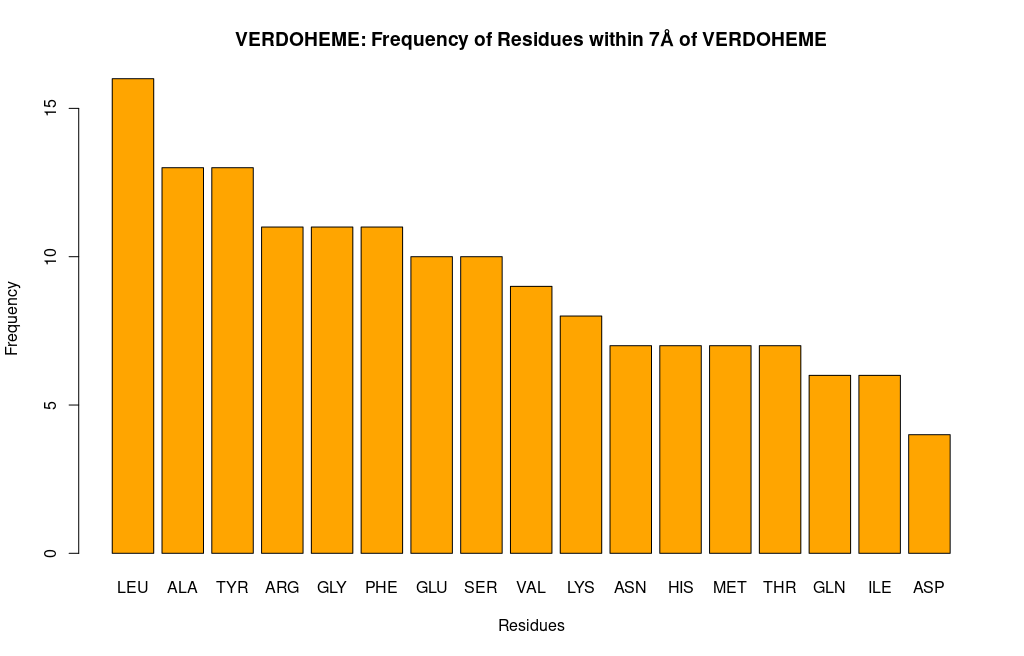
\includegraphics{figures/fuckinghell.png}
	\end{figure}
	
				%\%begin{figure}
					%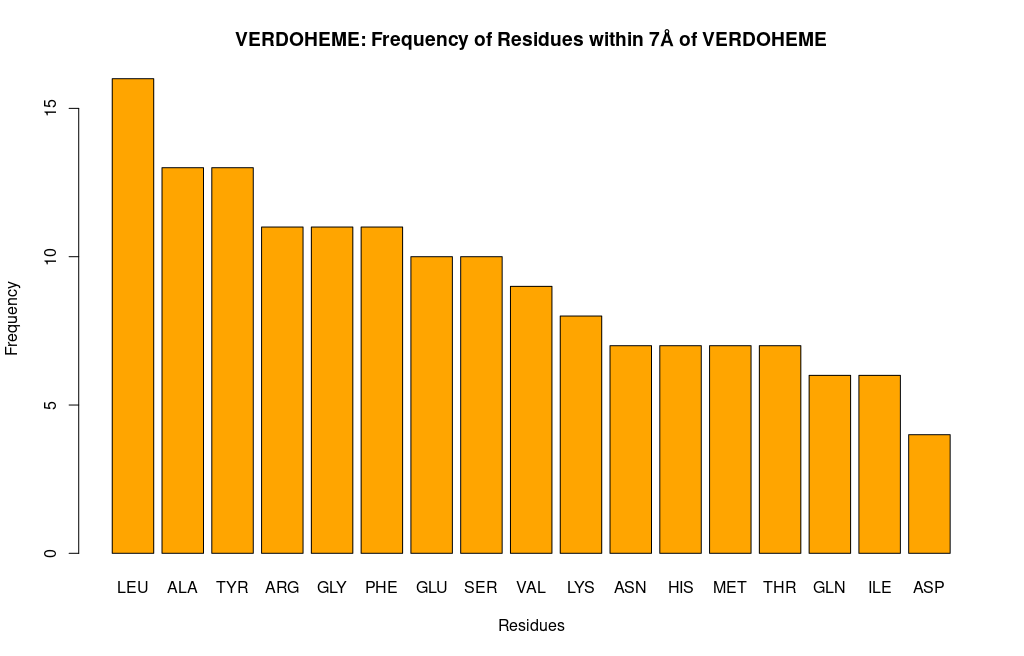
\includegraphics{figures/fuckinghell}
				\section{aafreqfigs}
	
	\begin{figure}
		\caption{within cells interlinked}
		\label{figs:HEM_aafreq}
		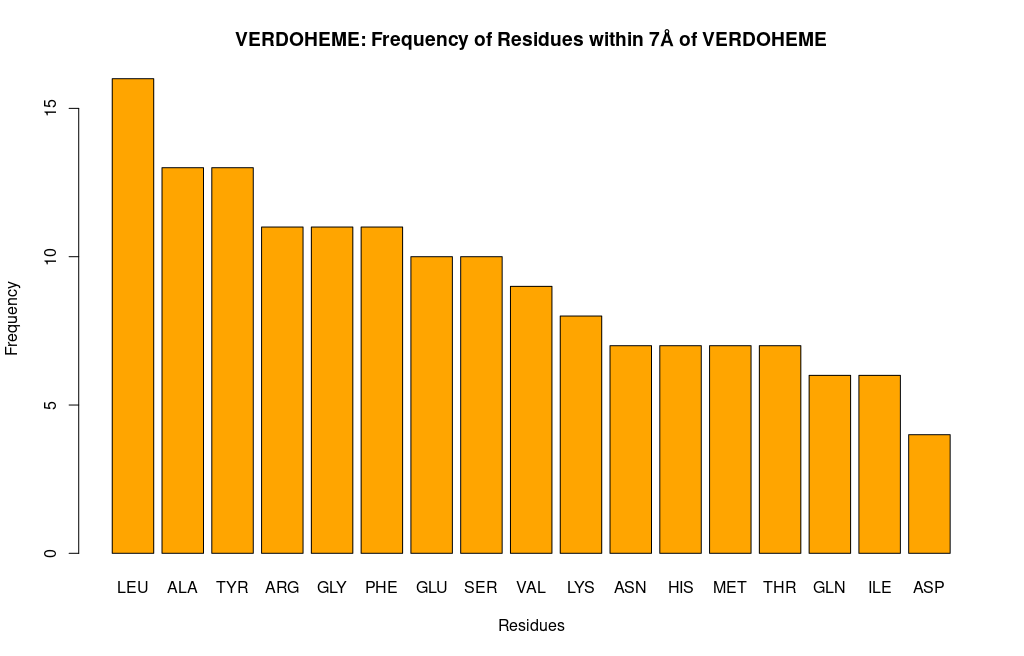
\includegraphics{figures/fuckinghell.png}
	\end{figure}
	
				%\end{figure}
				
		\chapter{Volume}
			\section{Tables}
			\section{Figures}
		% etc...
	\end{appendices}
	
	%[heading=subbibintoc]
	%add your sources in the bib file and change the style here
	%\bibliographystyle{alpha}
	%\bibliography{bibliography}
	
	%\printglossary[type=\acronymtype]
	%\printglossary
	
	%\cleardoublepage{}
	%\pagebreak
	
	%add your end matter here
	%\appendix{}
	
	%\input{C) Back Matter/appendix}
	
\end{document}